\documentclass[11pt,a4paper]{article}
\usepackage{fontspec}
\setmainfont{TeX Gyre Pagella}
\newfontfamily\headfont{Inter}[UprightFont=*-ExtraBold,BoldFont=*-ExtraBold,Extension=.otf,Path=/usr/share/fonts/opentype/inter/]
\usepackage[a4paper,margin=2.3cm]{geometry}
\usepackage{graphicx,booktabs,float,caption,array,xcolor,longtable}
\usepackage{xurl}
\usepackage[hidelinks]{hyperref}
\usepackage{titlesec}
\usepackage[round]{natbib}
\usepackage{setspace}
\setstretch{1.05}
\renewcommand{\topfraction}{0.9}
\renewcommand{\bottomfraction}{0.8}
\renewcommand{\textfraction}{0.1}
\renewcommand{\floatpagefraction}{0.75}
\setlength{\parindent}{0pt}
\setlength{\parskip}{0.55em}
\titleformat{\section}{\headfont\Large}{\thesection}{0.8em}{}
\titleformat{\subsection}{\headfont\large}{\thesubsection}{0.8em}{}
\captionsetup{font=small,labelfont=bf}
\urlstyle{same}
\hypersetup{pdftitle={Every Storm since 1851: Where Tropical Cyclones Form, Where They Hit, and Whether They Are Getting Stronger},pdfauthor={Tristan Hotham}}

\begin{document}
\begin{center}
{\Large\bfseries Every Storm since 1851: Where Tropical Cyclones Form, Where They Hit, and Whether They Are Getting Stronger\par}
\vspace{0.4em}
{\large A map and an honest reading of NOAA's global best track archive (IBTrACS)\par}
\vspace{1.2em}
{\large Tristan Hotham\par}
\vspace{0.3em}
{\small Independent researcher\\
ORCID: 0000-0003-4931-9349\\
DOI: https://doi.org/10.5281/zenodo.23858051\par}
\vspace{0.8em}
2026
\end{center}

\begin{quote}
\small
\begin{center}\textbf{Abstract}\end{center}
I map every tropical cyclone in NOAA's International Best Track Archive for Climate Stewardship (IBTrACS v04r01), 13,186 storms and depressions from 1851 to 2025, and use the archive to describe where storms form, where they make landfall and whether they are getting stronger, with attention to how the record itself has changed. Since 1980, 89.1 storms a year have reached tropical storm strength and 47.3 hurricane strength, with no clear trend in the number. Only 3.8\% of storms form within 5 degrees of the equator. Intersecting every six-hourly segment with Natural Earth coastlines, I find that from 1980 to 2025 China was hit by the most storms (263), the Philippines by the most at typhoon strength (129) and Category 3 or more (67), and that Guangdong is the most-hit coast (118). Using only the US agencies' 1-minute winds, the share of storms reaching Category 4 or 5 rose from 16.8\% in 1980 to 2002 to 21.2\% in 2003 to 2025 (two-proportion test $p$ $<$ 0.001), while the share reaching Category 3 or more did not change clearly. The latitude of peak intensity moved poleward by 45 km a decade in the Northern Hemisphere (95\% interval 17 to 72), driven by the western North Pacific. Before about 1970 the record misses many storms, especially weak ones far from land, so long-run comparisons are not reliable, and some of the recent intensity change may reflect changing measurement.

\textbf{Keywords:} tropical cyclones; hurricanes; typhoons; IBTrACS; landfall; Saffir-Simpson scale; best track data; observation bias; data visualisation
\end{quote}

\section{Introduction}
Tropical cyclones (hurricanes in the Atlantic and eastern Pacific, typhoons in the western Pacific, cyclones in the Indian Ocean and the South Pacific) are the most destructive storms on Earth. Their tracks have been recorded by many agencies over a century and a half, and IBTrACS, maintained by NOAA's National Centers for Environmental Information, merges those records into a single global archive \citep{knapp2010,gahtan2024}. This paper does three simple things with it. It maps every track by strength; it counts where storms form and where they come ashore; and it asks whether storms are getting stronger, using the part of the record that can answer that question fairly.

That last question is often asked of best track data and often answered badly. The archive is a record of observation as much as of storms: before satellites, a storm was recorded only if it reached land or a ship met it \citep{wikitc}, and the methods used to estimate intensity have changed several times. Much of the work here is therefore about separating the storms from the seeing. An interactive version, with every track, landfall and number, is at \url{https://maps.tristanhotham.com/hurricane-tracks/}.

\section{Data}
\textbf{IBTrACS.} I use version 4, revision v04r01, all basins, reduced to the synoptic six-hourly positions (00, 06, 12 and 18 UTC): 357,517 rows. I keep the main tracks and the provisional tracks of the most recent storms (those not yet reanalysed) and drop the ``spur'' tracks that IBTrACS uses for alternative positions around splits and mergers, leaving 352,746 positions of 13,289 storms. Seasons follow IBTrACS: a Southern Hemisphere season is named after the year in which it ends. The analyses use complete seasons 1851 to 2025 (13,186 systems); 2026 appears on the map only. IBTrACS is NOAA data with no copyright restrictions.

\textbf{Winds.} The Saffir-Simpson scale is defined on the 1-minute sustained wind at 10 m \citep{wikiss}. IBTrACS gives the 1-minute wind of the US agencies (the National Hurricane Center, the Central Pacific Hurricane Center and the Joint Typhoon Warning Center) as USA\_WIND, and the wind of the responsible regional agency as WMO\_WIND, which is often a 10-minute average and reads lower. I use USA\_WIND throughout and fall back on WMO\_WIND only for map colours, counts of storms reaching 34 knots and landfall strength. Categories are: tropical depression below 34 kt, tropical storm 34 to 63 kt, Category 1 from 64 kt, 2 from 83, 3 from 96, 4 from 113 and 5 from 137 kt. 5,568 systems (42\%) have no wind at all; almost all are from before the 1940s outside the North Atlantic.

\textbf{Geography.} Natural Earth 1:10m countries and states and provinces (public domain) for landfalls; 1:50m land for the figures.

\section{Methods}
\textbf{Basins} are those of IBTrACS at a storm's first position (central Pacific storms are counted with the eastern Pacific). \textbf{Genesis} is the first position of each storm that reached 34 kt. \textbf{Landfall:} each six-hourly segment is drawn as a straight line in longitude and latitude and intersected with every land polygon of Natural Earth's countries, so that islands count. A landfall is a point where a segment enters land from the sea (a point 3 km back along the segment must be at sea, which drops crossings of land borders), while the storm is not yet extratropical (NATURE not ET). Its time, position and wind are interpolated along the segment. A storm counts once per country, and once per state or province, at its strongest landfall there. Natural Earth counts France's overseas departments as France; I report them under their own names.

\textbf{Intensity shares} are the proportion of storms whose USA\_WIND reached 34 kt that went on to reach 96 kt (Category 3) or 113 kt (Category 4). \textbf{Latitude of lifetime maximum intensity} is the absolute latitude of the first position at which a storm's USA\_WIND peaks, averaged by season and hemisphere, following \citet{kossin2014}. \textbf{Accumulated cyclone energy} is the sum of the squared USA\_WIND, in units of $10^4$ kt$^2$, over six-hourly positions of 35 kt or more while tropical or subtropical.

\textbf{Trends} are ordinary least-squares lines through seasonal values, 1980 to 2025, with 95\% intervals from 4,000 bootstrap resamples of seasons; I also compare the halves 1980 to 2002 and 2003 to 2025 with a two-proportion $z$ test. I start in 1980 because geostationary satellites then covered the whole tropics; polar-orbiting satellites became operational in 1965, and the Dvorak technique for estimating intensity from satellite images was developed in the 1970s \citep{wikitc}.

\section{Results}
\subsection{The map}
Figure~\ref{fig:map} shows every track from 1851 to 2025. The western North Pacific dominates, with the densest and strongest tracks on Earth; the grey tracks over the Bay of Bengal, the Arabian Sea and the South Indian Ocean are the long early records of those basins, which have positions but no winds.

\begin{figure}[tbp]\centering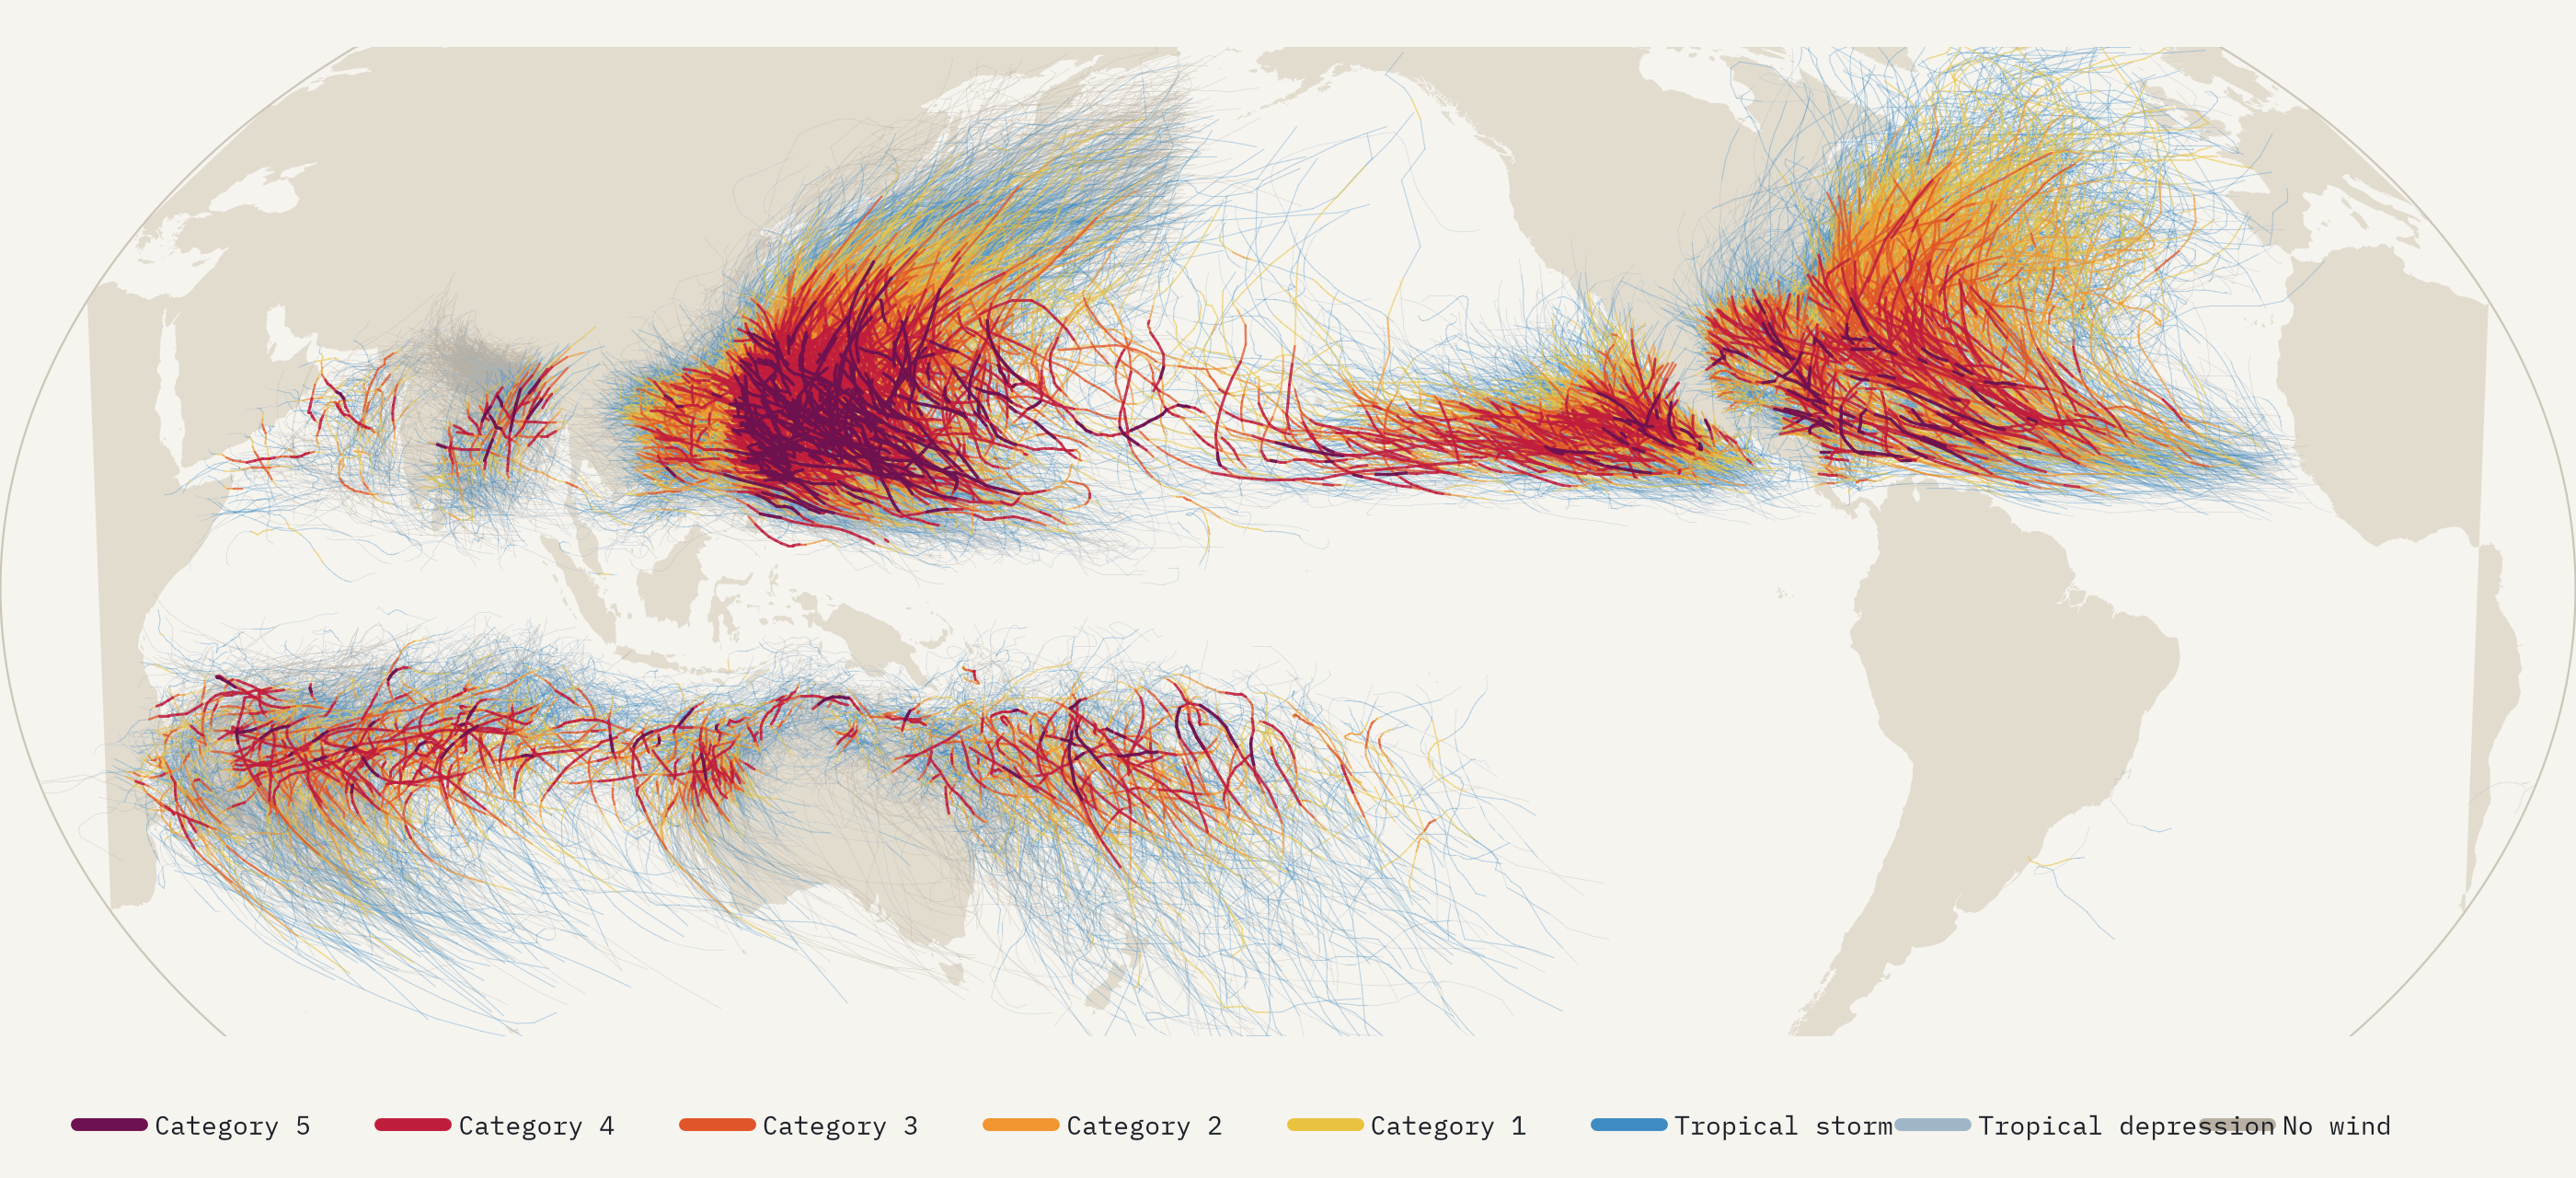
\includegraphics[width=\textwidth]{f_map.png}\caption{Every tropical cyclone track in IBTrACS v04r01, 1851 to 2025, coloured by Saffir-Simpson category at each six-hourly position (1-minute wind of the US agencies where given, else the agency wind). Equal Earth projection centred on 160°W.}\label{fig:map}\end{figure}

\subsection{How many storms, and how many were seen}
Since 1980 an average of 89.1 storms a season reached tropical storm strength (range 73 in 1991 to 106 in 2005), 47.3 reached hurricane strength and 16.5 Category 4 or more. The trend in the number of tropical storms is +1.1 a decade (95\% interval -0.8 to +2.9), in hurricanes -0.6 (-1.9 to +0.6). The western North Pacific contributes 28.6\% of tropical storms, the eastern Pacific 19.9\%, the South Indian 18.7\%, the North Atlantic 15.4\%, the South Pacific 11.7\% and the North Indian 5.7\%.

The long record (Figure~\ref{fig:peryear}) grows for reasons that have little to do with storms. Winds first appear in the eastern Pacific in 1902, the western Pacific in 1945, the South Pacific in 1956, the South Indian in 1957 and the North Indian in 1972; 15\% of the systems of the 1900s have a wind, against 99\% in the 1990s. In the North Atlantic, where winds go back to 1851, there were 7.5 tropical storms a season in 1851 to 1900 and 13.3 in 1976 to 2025, and 5.2 against 6.8 hurricanes. The difference is concentrated in the storms easiest to miss: only 11.5\% of the early storms never came within 500 km of land, against 23.0\% in the last fifty years. These figures describe the record, not a change in the climate.

\begin{figure}[tbp]\centering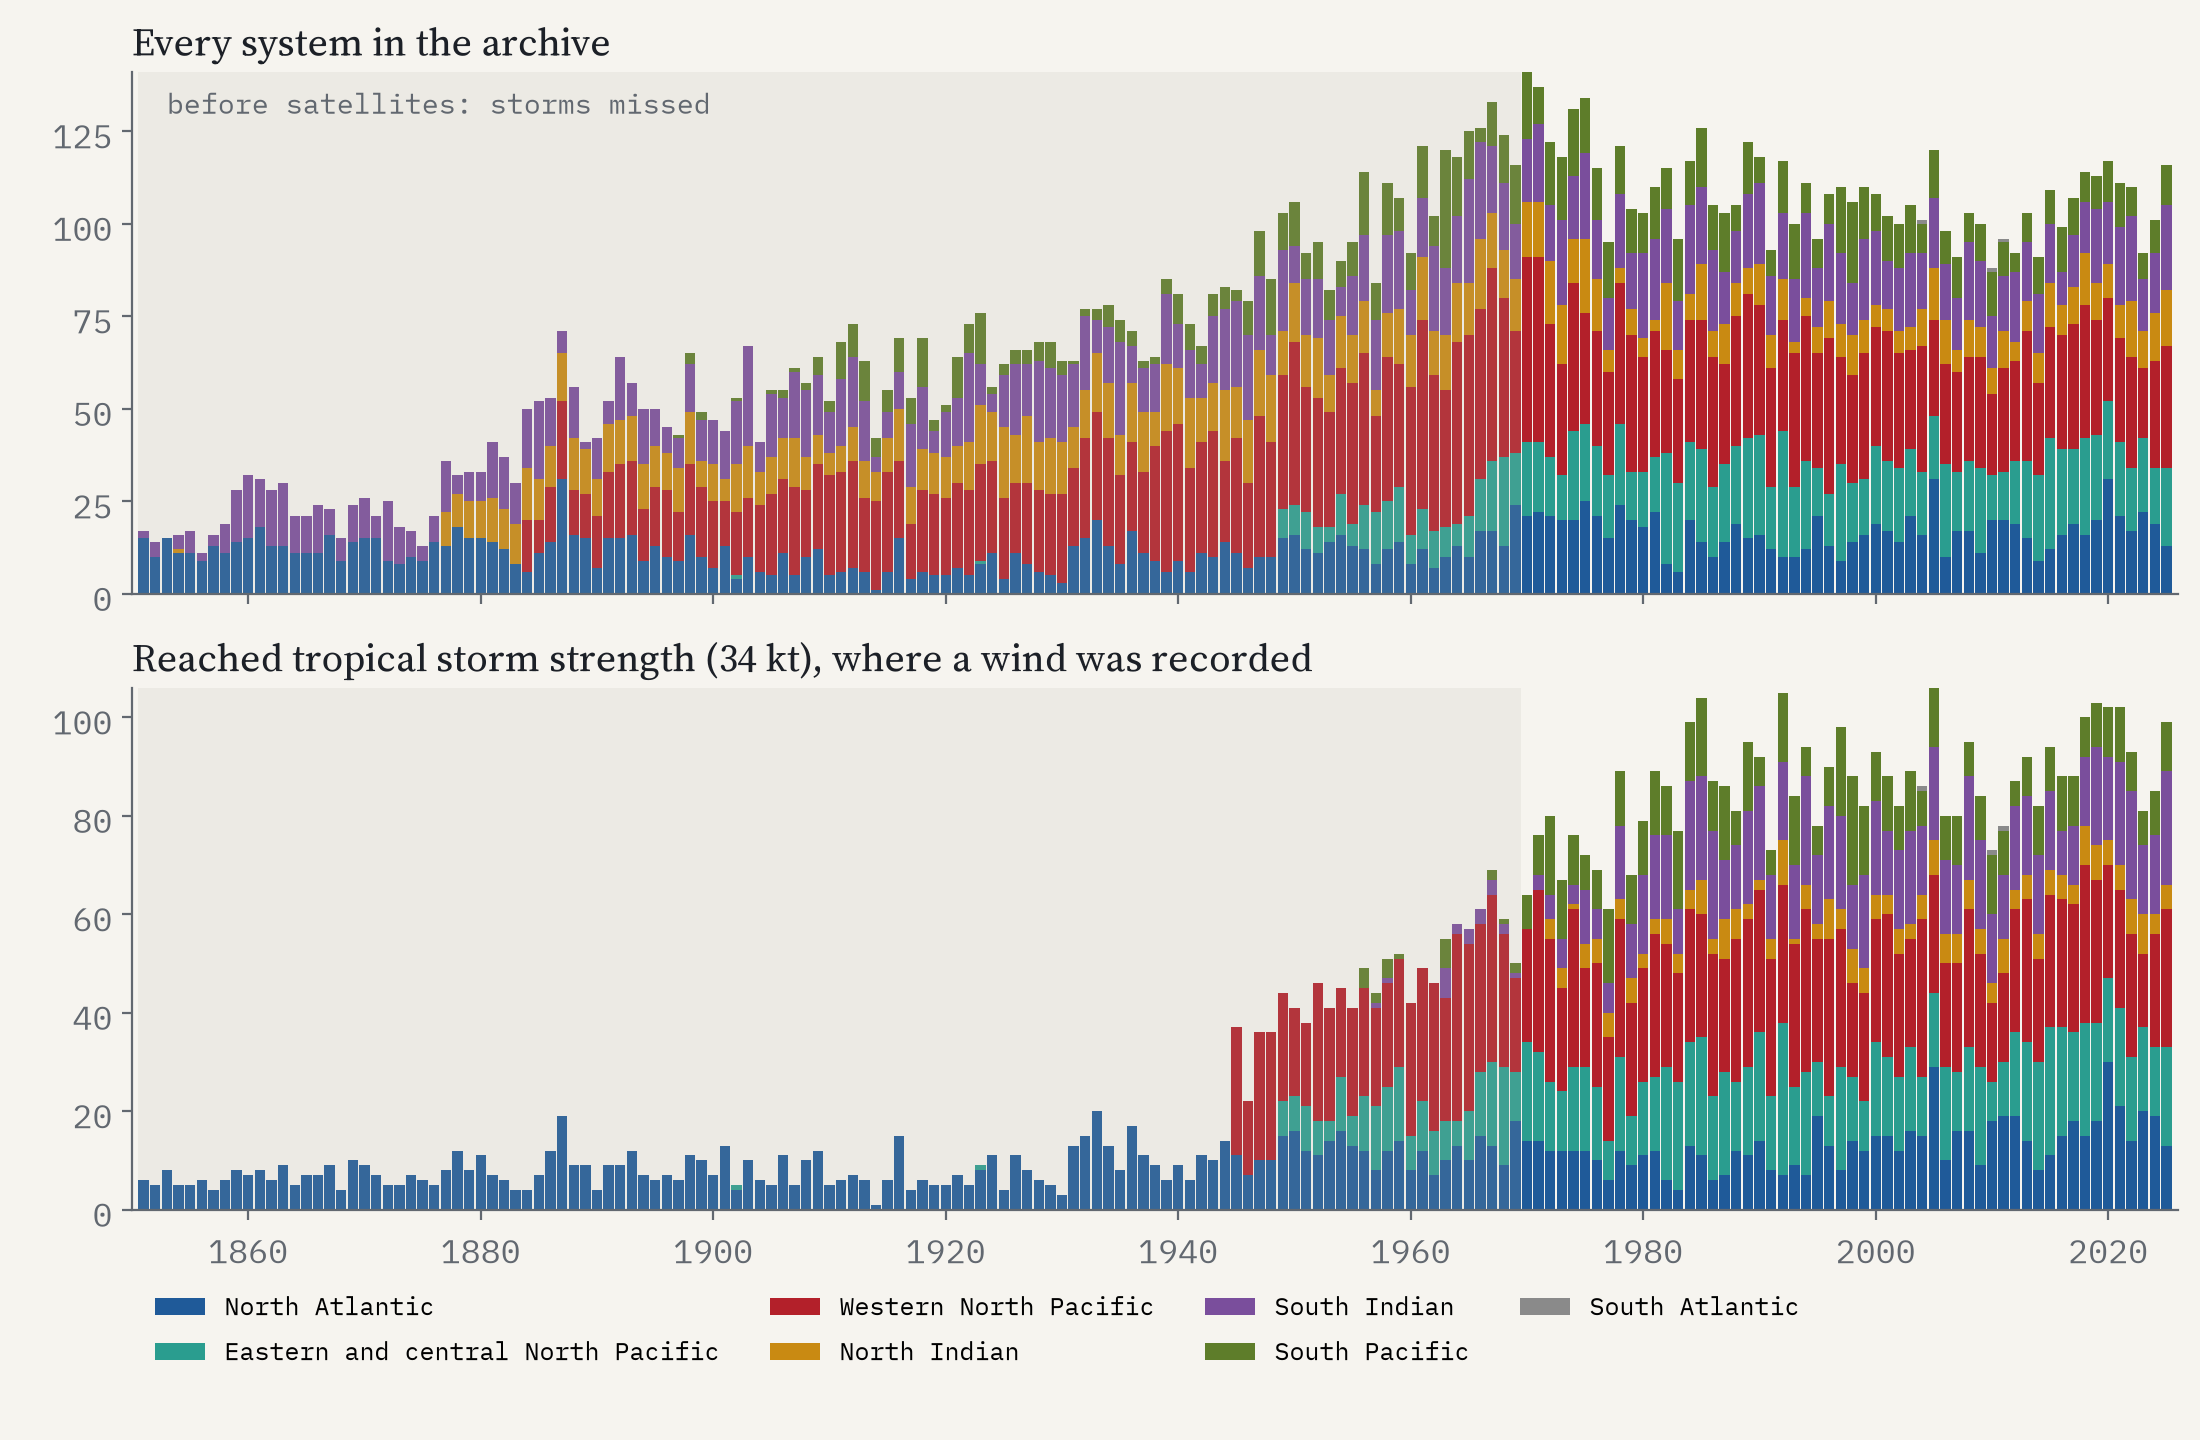
\includegraphics[width=\textwidth]{f_peryear.png}\caption{Systems per season by basin of formation: every system in the archive (top) and those that reached 34 kt where a wind was recorded (bottom). Shaded: before 1970.}\label{fig:peryear}\end{figure}

\subsection{Where storms form}
The 4,097 storms of 1980 to 2025 that reached 34 kt formed in two belts (Figure~\ref{fig:genesis}): 84.0\% between 5 and 20 degrees from the equator, only 3.8\% within 5 degrees, and 69.6\% in the Northern Hemisphere. The mean distance of genesis from the equator is 13.7 degrees. The densest 2.5 degree square is off southern Mexico, centred on 13.8°N, 101.2°W, with 7.6 storms a decade. The South Atlantic produced 3. Peak months are September in the North Atlantic, August in the eastern and western Pacific, January in the South Indian and February in the South Pacific; the North Indian Ocean has two seasons, peaking in May and November.

\begin{figure}[tbp]\centering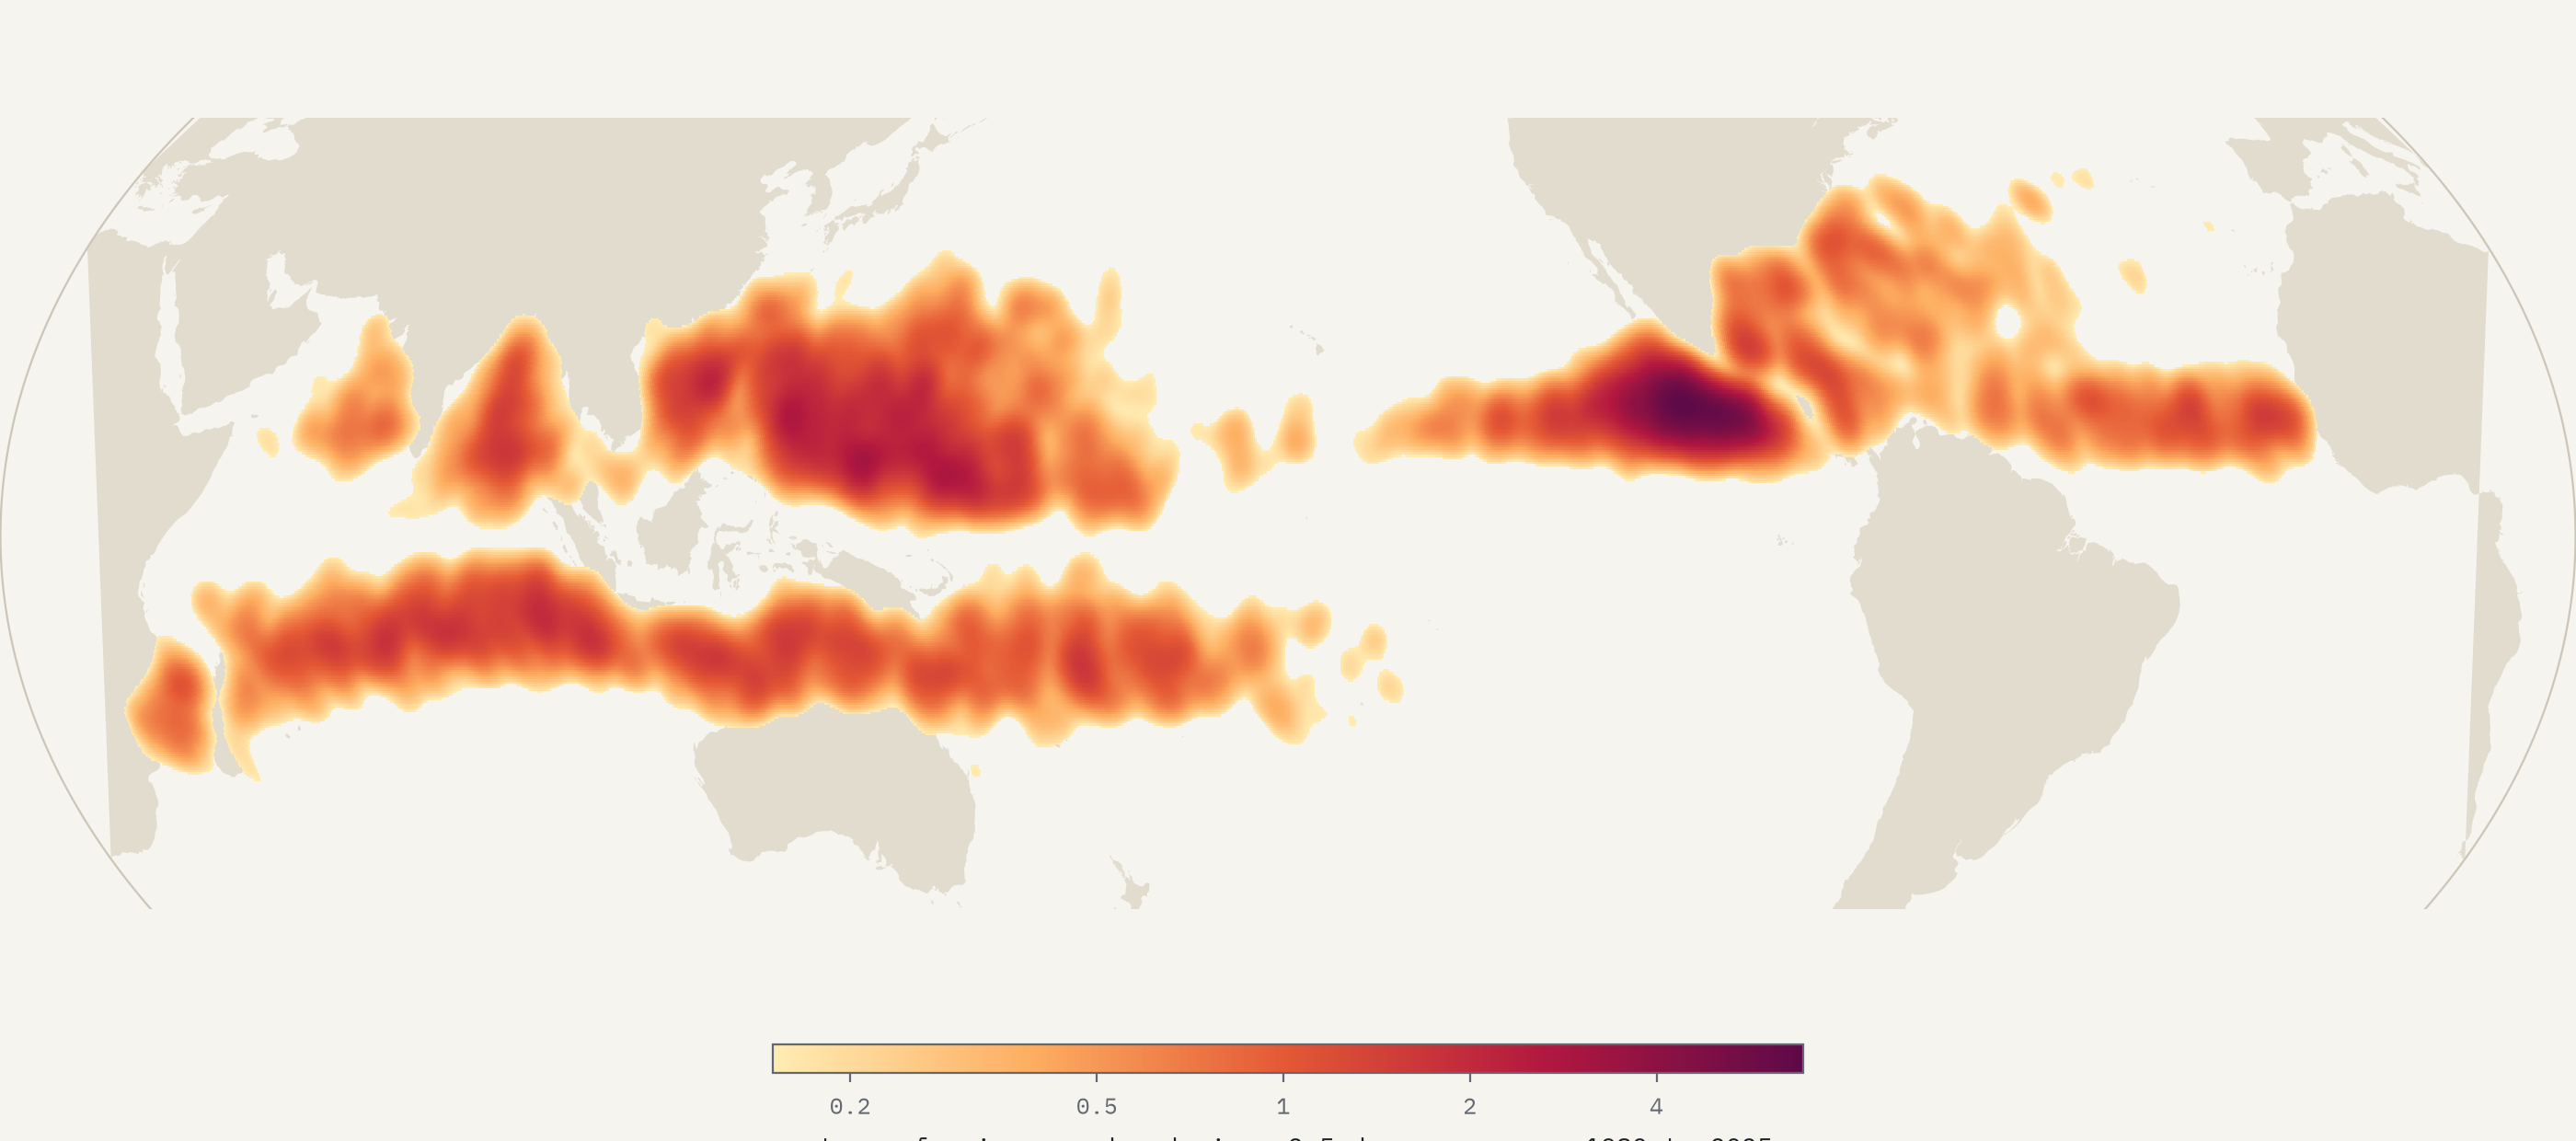
\includegraphics[width=\textwidth]{f_genesis.png}\caption{Where storms that reached 34 kt formed, 1980 to 2025: smoothed density (Gaussian kernel, 1.6 degrees), storms per decade per 2.5 degree square.}\label{fig:genesis}\end{figure}

\subsection{Where storms hit}
From 1980 to 2025, 40.1\% of tropical storms made landfall at tropical storm strength, and 35.0\% of hurricanes came ashore at hurricane strength, giving 2,158 storm and country landfalls in 94 countries and territories (Table~\ref{tab:countries}, Figure~\ref{fig:landfalls}). China leads in all landfalls, the Philippines in landfalls at typhoon strength and at Category 3 or more. Table~\ref{tab:regions} gives the most-hit states and provinces: Guangdong, Western Australia, Fujian, Queensland and Florida. Over the whole record, with winds where known, the United States has the most counted landfalls (565), a reflection of how long its coast has been watched.

Interpolating winds between six-hourly positions smooths sharp peaks, so landfall strength can read a category lower than the official value: Andrew (1992), officially a Category 5 landfall in Florida \citep{wikiss}, reads here as Category 4. The strongest landfalls by this measure are Haiyan on Leyte in 2013 (166 kt), Meranti on Batanes in 2016 (165 kt) and Dorian on the Abaco Islands in 2019 (160 kt).

\begin{figure}[tbp]\centering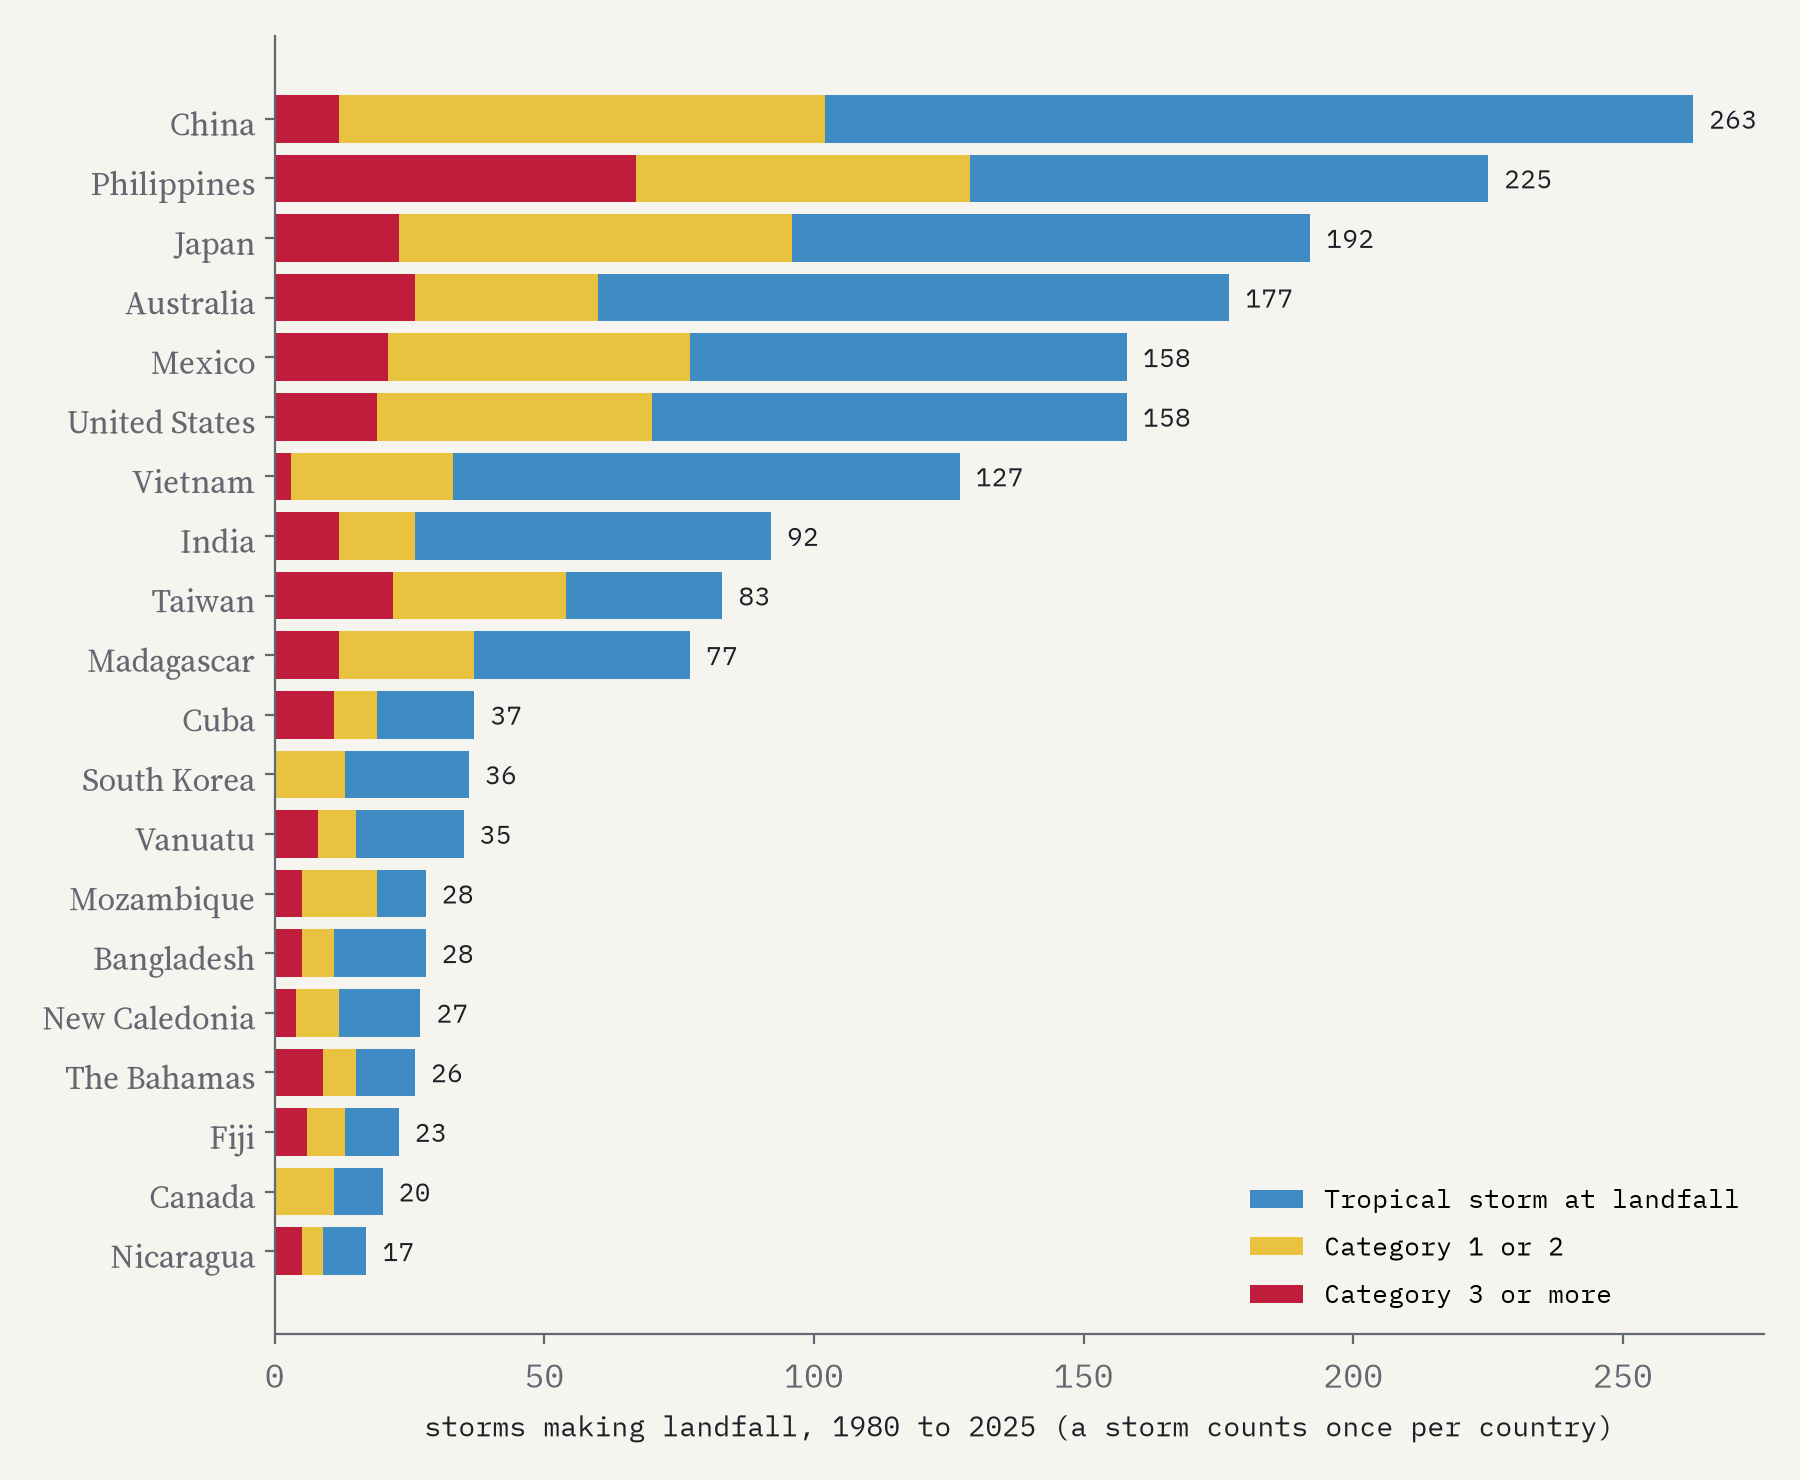
\includegraphics[width=.8\textwidth]{f_landfalls.png}\caption{The 20 countries with most landfalls, 1980 to 2025, by strength at landfall.}\label{fig:landfalls}\end{figure}

\begin{table}[tbp]\centering\small\caption{Countries and territories with most landfalls, 1980 to 2025: storms making landfall at least once, by strength at landfall (interpolated wind).}\label{tab:countries}\begin{tabular}{lrrrrr}\toprule Country & Tropical storm+ & Hurricane+ & Cat 3+ & Cat 5 & A year\\\midrule
China & 263 & 102 & 12 & 0 & 5.7\\
Philippines & 225 & 129 & 67 & 8 & 4.9\\
Japan & 192 & 96 & 23 & 0 & 4.2\\
Australia & 177 & 60 & 26 & 1 & 3.8\\
Mexico & 158 & 77 & 21 & 3 & 3.4\\
United States & 158 & 70 & 19 & 0 & 3.4\\
Vietnam & 127 & 33 & 3 & 0 & 2.8\\
India & 92 & 26 & 12 & 0 & 2.0\\
Taiwan & 83 & 54 & 22 & 0 & 1.8\\
Madagascar & 77 & 37 & 12 & 0 & 1.7\\
Cuba & 37 & 19 & 11 & 1 & 0.8\\
South Korea & 36 & 13 & 0 & 0 & 0.8\\
Vanuatu & 35 & 15 & 8 & 2 & 0.8\\
Mozambique & 28 & 19 & 5 & 0 & 0.6\\
Bangladesh & 28 & 11 & 5 & 0 & 0.6\\
New Caledonia & 27 & 12 & 4 & 0 & 0.6\\
The Bahamas & 26 & 15 & 9 & 2 & 0.6\\
Fiji & 23 & 13 & 6 & 1 & 0.5\\
Canada & 20 & 11 & 0 & 0 & 0.4\\
Nicaragua & 17 & 9 & 5 & 1 & 0.4\\
Myanmar & 16 & 9 & 4 & 0 & 0.3\\
Northern Mariana Islands & 15 & 6 & 3 & 1 & 0.3\\
Dominican Republic & 15 & 4 & 1 & 0 & 0.3\\
Belize & 14 & 5 & 1 & 0 & 0.3\\
New Zealand & 14 & 0 & 0 & 0 & 0.3\\
\bottomrule\end{tabular}\end{table}
\begin{table}[tbp]\centering\small\caption{The most-hit states, provinces and prefectures (Natural Earth admin 1), 1980 to 2025.}\label{tab:regions}\begin{tabular}{llrrr}\toprule Region & Country & Tropical storm+ & Hurricane+ & Cat 3+\\\midrule
Guangdong & China & 118 & 47 & 7\\
Western Australia & Australia & 96 & 37 & 19\\
Fujian & China & 65 & 26 & 2\\
Queensland & Australia & 61 & 15 & 5\\
Florida & United States & 58 & 21 & 10\\
Okinawa Prefecture & Japan & 55 & 35 & 16\\
Hainan & China & 49 & 21 & 2\\
Cagayan & Philippines & 47 & 28 & 15\\
Kagoshima Prefecture & Japan & 39 & 24 & 4\\
Northern Territory & Australia & 39 & 13 & 4\\
Aurora & Philippines & 34 & 21 & 12\\
Baja California Sur & Mexico & 34 & 15 & 2\\
Quezon & Philippines & 33 & 21 & 9\\
Zhejiang & China & 33 & 12 & 2\\
Louisiana & United States & 31 & 16 & 4\\
Texas & United States & 29 & 15 & 3\\
Andhra Pradesh & India & 29 & 7 & 5\\
Eastern Samar & Philippines & 28 & 11 & 4\\
Palawan & Philippines & 28 & 6 & 1\\
Taitung & Taiwan & 27 & 22 & 8\\
\bottomrule\end{tabular}\end{table}

\subsection{The strongest storms}
Table~\ref{tab:strongest} lists the strongest storms by peak 1-minute wind. Hurricane Patricia (2015) and Typhoon Nancy (1961) share the highest value, 185 kt; Wikipedia gives Patricia's as the highest sustained wind ever recorded \citep{wikitc}. 11 of the top 20 are western Pacific typhoons of the 1950s and 1960s, from the early decades of aircraft reconnaissance, whose winds are not directly comparable with modern estimates. The lowest pressure is Typhoon Tip's 870 hPa in 1979. 324 storms reached Category 5, 216 of them since 1980 and 209 in the western North Pacific.

\begin{table}[tbp]\centering\small\caption{The 20 strongest storms by peak 1-minute wind (US agencies), ties ordered by lowest pressure, with countries where they made landfall at tropical storm strength or more.}\label{tab:strongest}\begin{tabular}{lrp{3.6cm}rrp{4.2cm}}\toprule Storm & Season & Basin & kt & hPa & Landfalls\\\midrule
Patricia & 2015 & Eastern and central North Pacific & 185 & 872 & Mexico\\
Nancy & 1961 & Western North Pacific & 185 & 890 & Japan, Russia\\
Violet & 1961 & Western North Pacific & 180 & 895 & Japan\\
Ruth & 1955 & Western North Pacific & 180 & 925 & none\\
Ida & 1958 & Western North Pacific & 175 & 877 & Guam, Japan\\
Kit & 1966 & Western North Pacific & 170 & 880 & none\\
Joan & 1959 & Western North Pacific & 170 & 885 & Taiwan, China\\
Meranti & 2016 & Western North Pacific & 170 & 890 & Philippines, Taiwan, China\\
Sally & 1964 & Western North Pacific & 170 & 895 & Guam, Philippines, China\\
Haiyan & 2013 & Western North Pacific & 170 & 895 & Philippines, Vietnam\\
Surigae & 2021 & Western North Pacific & 170 & 895 & none\\
Opal & 1964 & Western North Pacific & 170 & 900 & Philippines\\
Goni & 2020 & Western North Pacific & 170 & 905 & Philippines\\
Tip & 1979 & Western North Pacific & 165 & 870 & Japan, Russia\\
Melissa & 2025 & North Atlantic & 165 & 892 & Jamaica, Cuba, The Bahamas\\
Vera & 1959 & Western North Pacific & 165 & 895 & Japan\\
Allen & 1980 & North Atlantic & 165 & 899 & United States\\
Mawar & 2023 & Western North Pacific & 165 & 900 & Japan\\
Grace & 1958 & Western North Pacific & 165 & 905 & China\\
Sarah & 1959 & Western North Pacific & 165 & 905 & Japan, South Korea, Russia\\
\bottomrule\end{tabular}\end{table}

\subsection{Are storms getting stronger?}
Figure~\ref{fig:shares} and Table~\ref{tab:shares} show the share of storms reaching Category 3+ and 4+. Worldwide the Category 4+ share was 12.5\% in the 1980s, 20.6\% in the 1990s, 20.2\% in the 2000s, 22.8\% in the 2010s and 18.5\% in 2020 to 2025. Between the halves of the satellite era it rose from 16.8\% to 21.2\% ($p$ $<$ 0.001; trend in the annual share +2.0 percentage points a decade, 95\% interval +0.7 to +3.3), and the Category 5 share from 4.3\% to 6.5\% ($p$ = 0.003). The number of Category 4+ storms a season rose by 2.0 a decade (0.8 to 3.1). The Category 3+ share changed less: 26.7\% against 28.4\% ($p$ = 0.21; trend +0.7, interval -0.6 to +2.1). Accumulated cyclone energy shows no clear trend (-7.7 a decade, -45.1 to +25.0).

By basin, the Category 4+ share rose clearly in the South Pacific, the western North Pacific and the South Indian Ocean, and not clearly in the North Atlantic, the eastern Pacific or the North Indian Ocean. Two cautions apply. Most of the global rise happened between the 1980s and the 1990s, the period in which satellite intensity methods were maturing, so part of it may be measurement. And the North Atlantic's long record (a Category 3+ share of 16.1\% in 1851 to 1900 against 21.0\% in 1976 to 2025) is not a fair comparison, because many storms, and especially weaker ones far from land, were missed. These results are consistent in direction with the global increase in the proportion of major storms from 1979 to 2017 reported by \citet{kossin2020} and summarised by \citet{wikitc}; in this raw best-track version the signal is clear for Category 4 and above but not for Category 3 and above.

\begin{figure}[tbp]\centering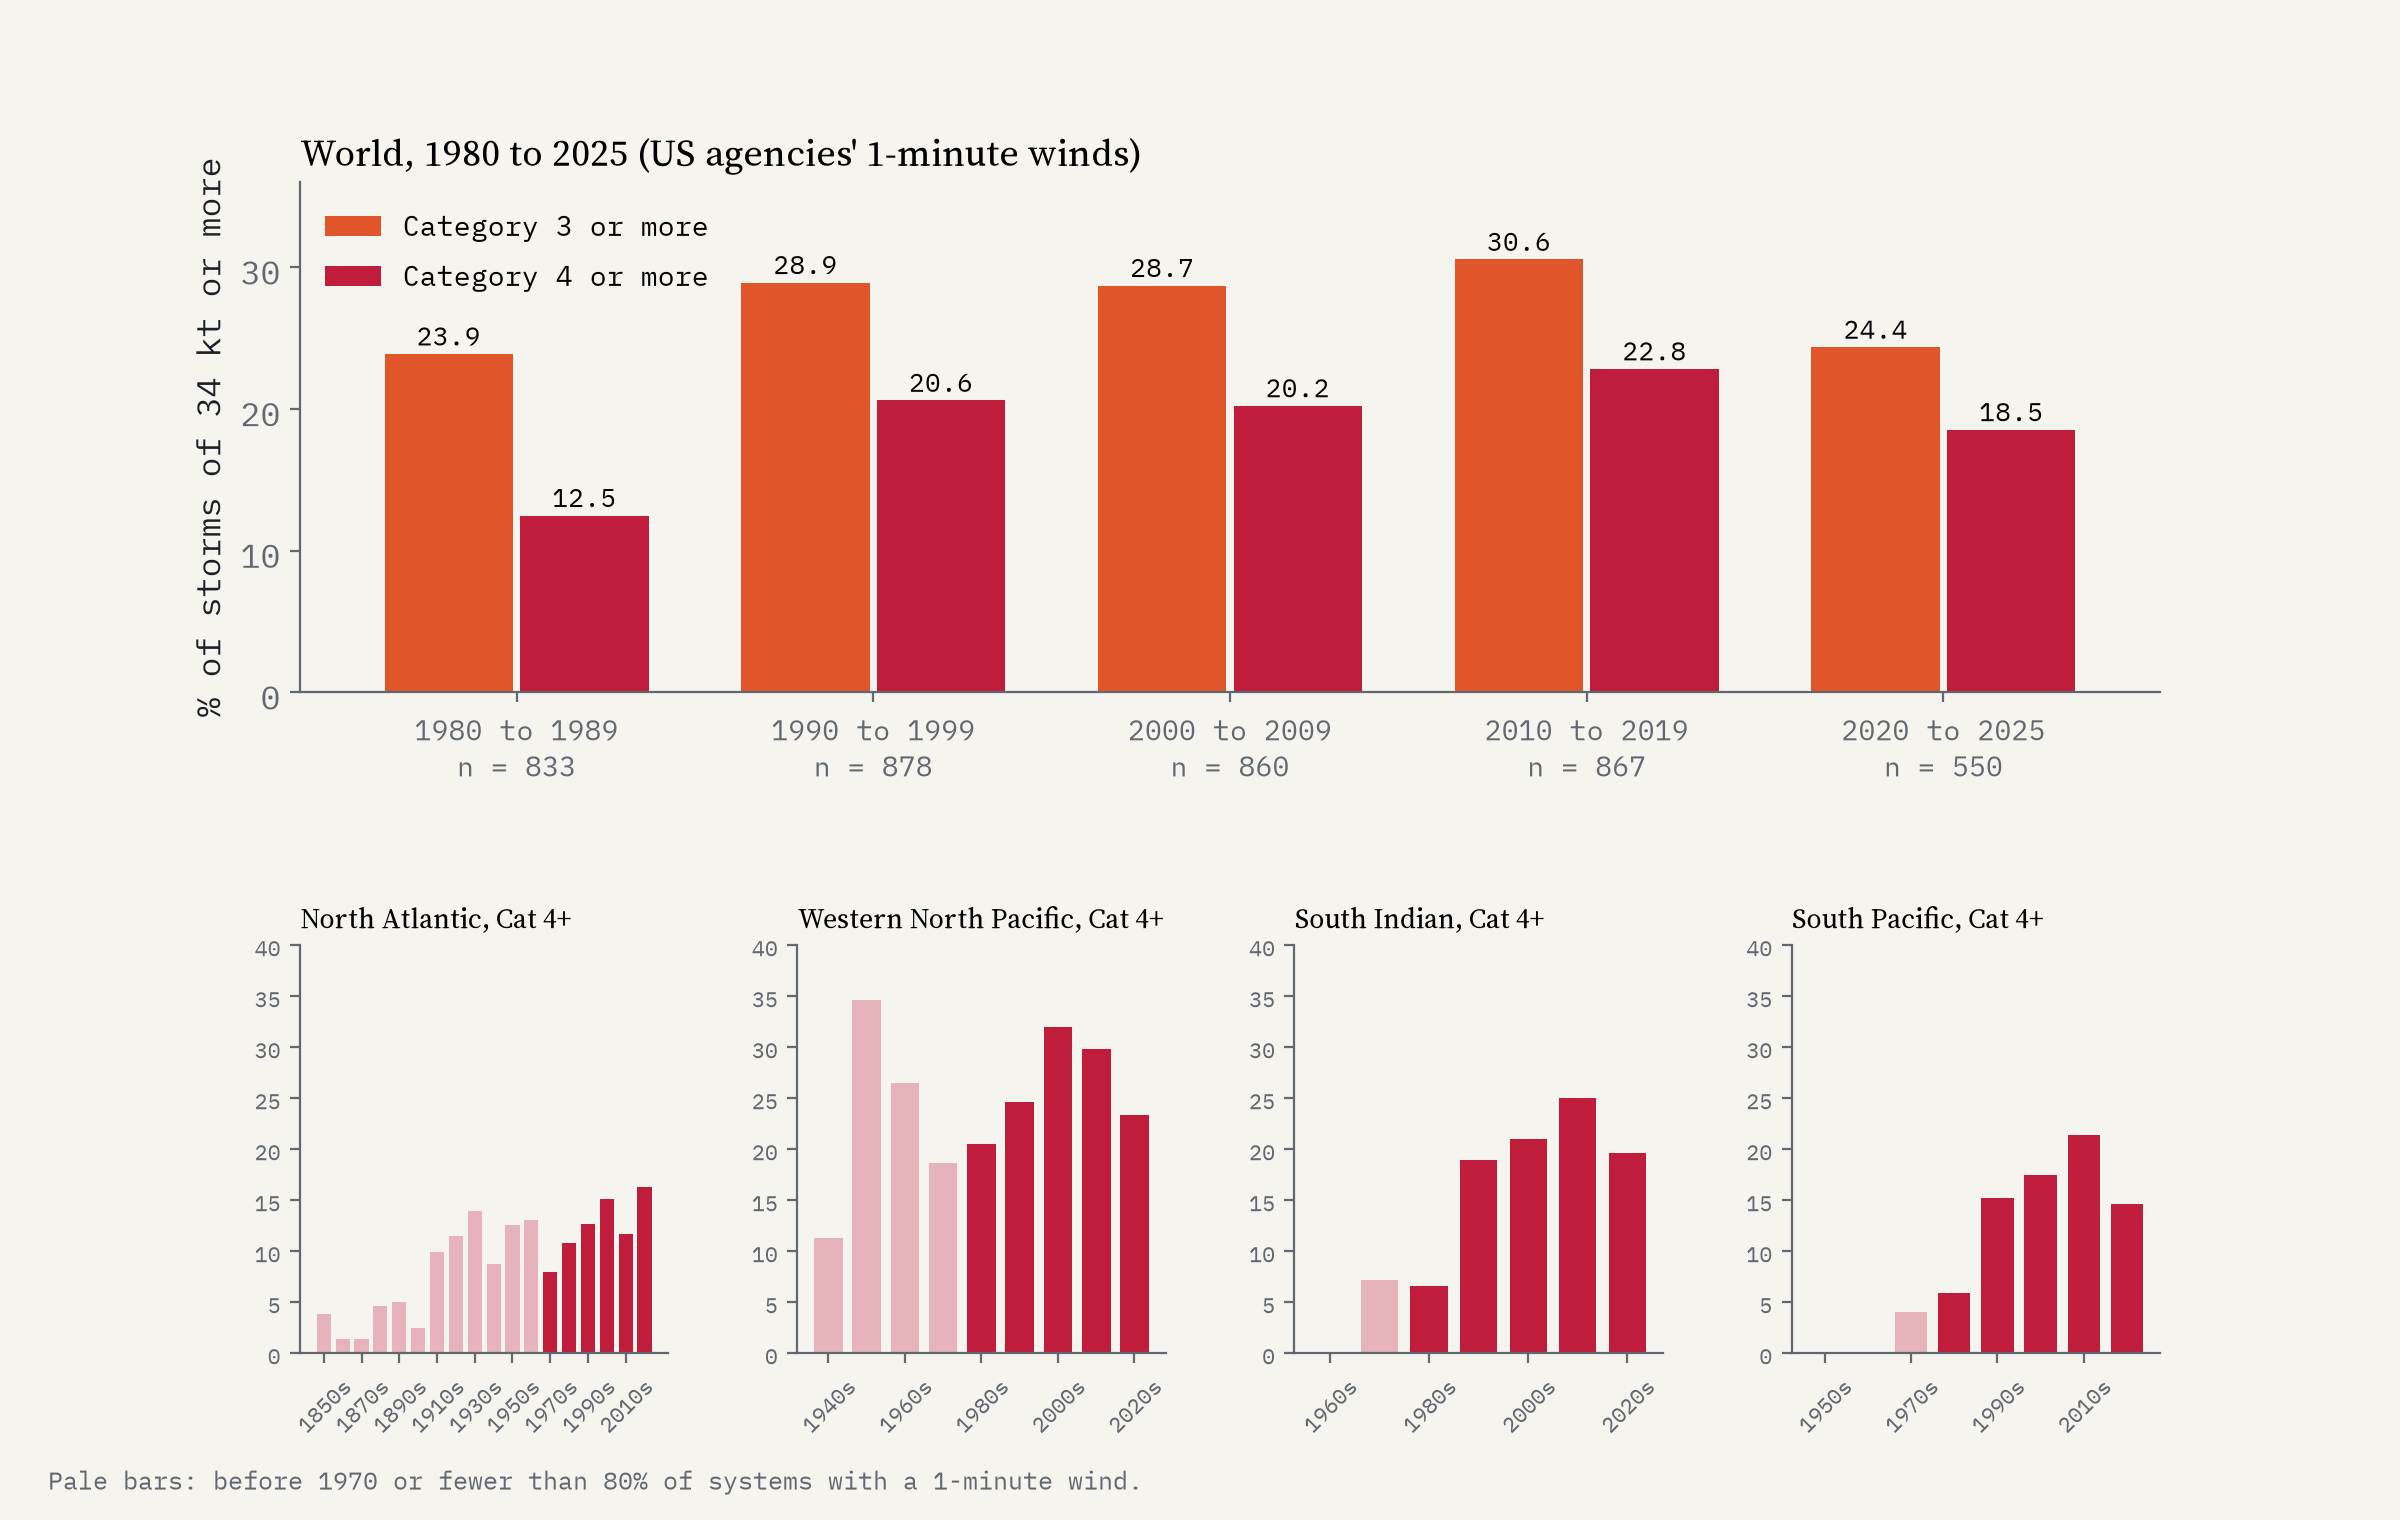
\includegraphics[width=\textwidth]{f_shares.png}\caption{Share of storms reaching Category 3+ and 4+ by decade, worldwide 1980 to 2025 (top), and Category 4+ in four basins over their whole record (bottom). Pale bars: before 1970, or fewer than 80\% of systems with a 1-minute wind.}\label{fig:shares}\end{figure}

\begin{table}[tbp]\centering\small\caption{Share of storms (34 kt or more, US 1-minute wind) reaching Category 3+ and 4+, 1980 to 2002 against 2003 to 2025, with two-proportion test $p$-values.}\label{tab:shares}\begin{tabular}{p{4.6cm}rrrrrrr}\toprule Basin & $n$ & Cat 3+ \% & & $p$ & Cat 4+ \% & & $p$\\ & & first & second & & first & second & \\\midrule
North Atlantic & 246 / 383 & 20.7 & 21.4 & 0.839 & 11.8 & 14.4 & 0.355\\
Eastern and central North Pacific & 410 / 404 & 29.8 & 25.5 & 0.174 & 19.0 & 19.1 & 0.990\\
Western North Pacific & 605 / 551 & 31.9 & 35.8 & 0.166 & 23.0 & 29.8 & 0.009\\
North Indian & 102 / 124 & 12.7 & 19.4 & 0.181 & 7.8 & 12.1 & 0.293\\
South Indian & 361 / 355 & 26.6 & 31.0 & 0.194 & 15.0 & 21.1 & 0.032\\
South Pacific & 241 / 203 & 20.3 & 29.1 & 0.033 & 9.5 & 20.7 & $<$0.001\\
\midrule World & 1965 / 2023 & 26.7 & 28.4 & 0.215 & 16.8 & 21.2 & $<$0.001\\
\bottomrule\end{tabular}\end{table}

\subsection{The poleward shift of peak intensity}
The average latitude at which storms reach their peak moved poleward from 1980 to 2025 (Figure~\ref{fig:lmi}, Table~\ref{tab:lmi}): by 45 km a decade in the Northern Hemisphere (17 to 72), 21 km in the Southern (3 to 40; OLS $p$ = 0.06), and 40 km over both. The western North Pacific drives it (65 km a decade, 33 to 96); the North Atlantic moved, not clearly, the other way (-53 km, -103 to 4). This agrees in direction with \citet{kossin2014}.

\begin{figure}[tbp]\centering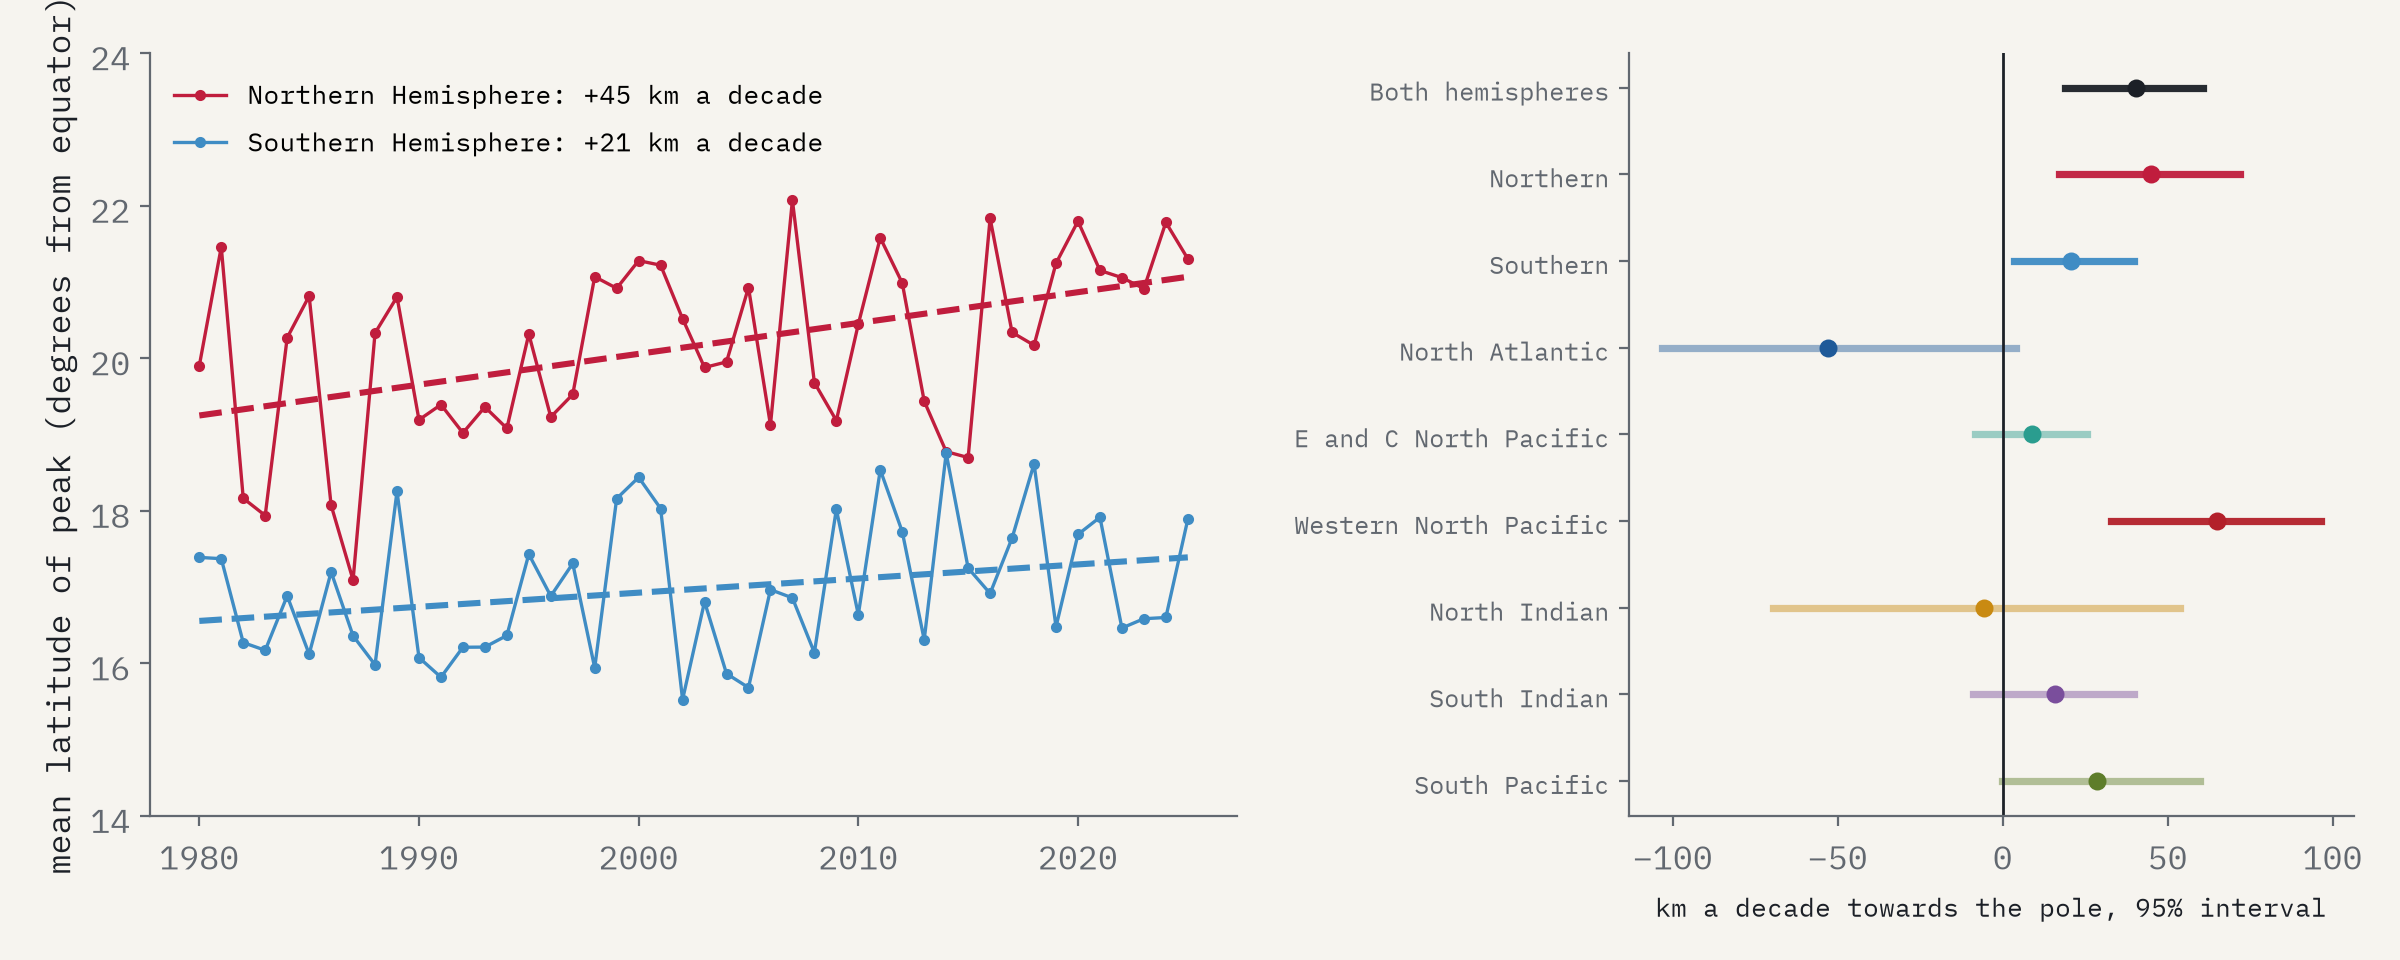
\includegraphics[width=\textwidth]{f_lmi.png}\caption{Left: mean absolute latitude of lifetime maximum intensity per season and hemisphere, with least-squares trends. Right: trends by hemisphere and basin, km a decade, with 95\% bootstrap intervals (pale where the interval includes zero).}\label{fig:lmi}\end{figure}

\begin{table}[tbp]\centering\small\caption{Trend in the latitude of lifetime maximum intensity, 1980 to 2025, km a decade (positive: towards the pole), with 95\% bootstrap intervals and OLS $p$-values.}\label{tab:lmi}\begin{tabular}{lrrr}\toprule & km a decade & 95\% interval & $p$\\\midrule
Both hemispheres & +40 & +19 to +61 & 0.000\\
Northern Hemisphere & +45 & +17 to +72 & 0.001\\
Southern Hemisphere & +21 & +3 to +40 & 0.057\\
North Atlantic & -53 & -103 to +4 & 0.087\\
Eastern and central North Pacific & +9 & -8 to +26 & 0.373\\
Western North Pacific & +65 & +33 to +96 & 0.000\\
North Indian & -6 & -70 to +54 & 0.858\\
South Indian & +16 & -9 to +40 & 0.175\\
South Pacific & +29 & -0 to +60 & 0.146\\
\bottomrule\end{tabular}\end{table}

\section{Limitations}
The archive is heterogeneous: agencies, instruments and methods differ by basin and decade, and IBTrACS merges rather than homogenises them. Before about 1970 many storms are missing, especially weak, short-lived ones far from land, and outside the North Atlantic there are no winds before the 1940s or later; I therefore compare intensity only from 1980, and even then satellite methods changed. The 2025 season includes provisional tracks. Six-hourly positions and straight segments cut corners and can miss small islands; landfall winds are interpolated and often below official values. Natural Earth coastlines and boundaries are generalised. Nothing here separates natural variability (El Ni\~no, Atlantic multidecadal variability) from long-term change, and nothing here attributes trends to climate change.

\section{Conclusion}
The global record shows about 89 tropical storms a year since 1980 with no clear change in number, a clear rise in the share reaching Category 4 or 5, and a poleward shift in where storms peak, especially in the western Pacific. China is hit most often and the Philippines hardest. Before satellites the archive is a record of where people were watching as much as of where storms went, and it should be read that way.

\section*{Data and code availability}
The interactive map is at \url{https://maps.tristanhotham.com/hurricane-tracks/}. Data and code are at \url{https://github.com/Tristan-Hotham/hurricane-tracks} and archived with this paper at https://doi.org/10.5281/zenodo.23858051. Derived data are released under CC BY 4.0 and code under the MIT licence. IBTrACS is NOAA data with no copyright restrictions; please cite \citet{knapp2010} and \citet{gahtan2024}.

\section*{AI statement}
I wrote the text, with drafting and editing assistance from Claude (Anthropic), which also helped prepare the analysis code. I reviewed and checked all text and results.

\begin{thebibliography}{9}
\bibitem[Gahtan et al.(2024)]{gahtan2024} Gahtan, J., Knapp, K. R., Schreck, C. J., Diamond, H. J., Kossin, J. P. and Kruk, M. C. (2024) International Best Track Archive for Climate Stewardship (IBTrACS) Project, Version 4r01. NOAA National Centers for Environmental Information. Retrieved 2026.
\bibitem[Knapp et al.(2010)]{knapp2010} Knapp, K. R., Kruk, M. C., Levinson, D. H., Diamond, H. J. and Neumann, C. J. (2010) The International Best Track Archive for Climate Stewardship (IBTrACS): unifying tropical cyclone best track data. \emph{Bulletin of the American Meteorological Society} 91, 363 to 376.
\bibitem[Kossin et al.(2014)]{kossin2014} Kossin, J. P., Emanuel, K. A. and Vecchi, G. A. (2014) The poleward migration of the location of tropical cyclone maximum intensity. \emph{Nature} 509, 349 to 352.
\bibitem[Kossin et al.(2020)]{kossin2020} Kossin, J. P., Knapp, K. R., Olander, T. L. and Velden, C. S. (2020) Global increase in major tropical cyclone exceedance probability over the past four decades. \emph{Proceedings of the National Academy of Sciences} 117, 11975 to 11980.
\bibitem[Natural Earth(2026)]{naturalearth} Natural Earth (2026) Admin 0 countries, admin 1 states and provinces, land. Public domain. \url{https://www.naturalearthdata.com/}
\bibitem[Wikipedia(2026a)]{wikitc} Wikipedia contributors (2026a) Tropical cyclone. CC BY-SA 4.0. \url{https://en.wikipedia.org/wiki/Tropical_cyclone}
\bibitem[Wikipedia(2026b)]{wikiss} Wikipedia contributors (2026b) Saffir-Simpson scale. CC BY-SA 4.0. \url{https://en.wikipedia.org/wiki/Saffir\%E2\%80\%93Simpson_scale}
\end{thebibliography}
\end{document}
